\documentclass{standalone}
\usepackage{pgfplots}
\usepackage{amsmath}

\pgfplotsset{compat=newest}

\begin{document}
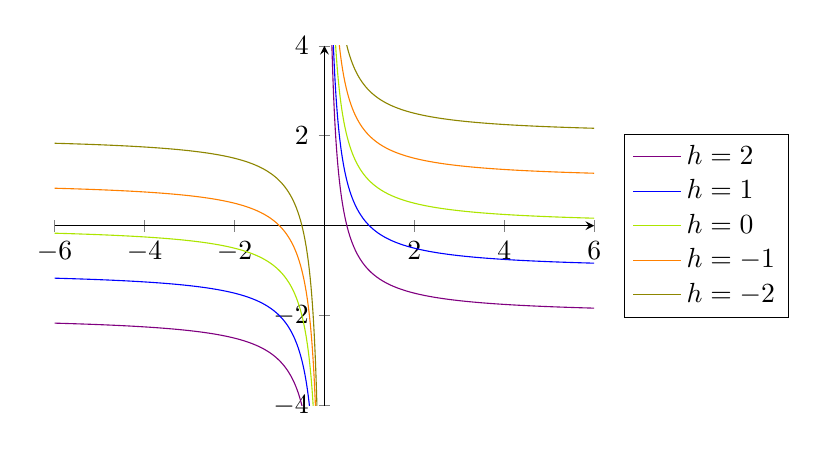
\begin{tikzpicture}
  \begin{axis}[
      axis lines= middle,
      xmin=-6,xmax=6,
      ymin=-4, ymax=4,
      axis equal image,
      trig format plots=rad,
      legend style={at={(axis cs:\xmax+2.5,0)},
          anchor=center,
          % /tikz/column 2/.style={
          %     column sep=5pt,
          %   },
        },
      legend cell align = {left},
      %legend columns=-1,
    ]
    \def\xmax{\pgfkeysvalueof{/pgfplots/xmax}}
    \def\xmin{\pgfkeysvalueof{/pgfplots/xmin}}
    \def\ymax{\pgfkeysvalueof{/pgfplots/ymax}}
    \def\ymin{\pgfkeysvalueof{/pgfplots/ymin}}
    %%%% y=0
    % \addplot [
    %   samples=10,
    %   black,
    %   dashed,
    %   domain=\xmin:\xmax,
    %   forget plot,
    % ] {0};

    %%%% k= 2
    \addplot [
      samples=400,
      smooth,
      violet,
      domain=\xmin:\xmax,
      restrict y to domain=-7:7,
    ] {1/x-2};

    %%%% k= 1
    \addplot [
      samples=400,
      smooth,
      blue,
      domain=\xmin:\xmax,
      restrict y to domain=-7:7,
    ] {1/x-1};

    %%%% k= 0
    \addplot [
      samples=400,
      smooth,
      lime!90!black,
      domain=\xmin:\xmax,
      restrict y to domain=-7:7,
    ] {1/x};

    %%%% k = -1
    \addplot [
      samples=400,
      smooth,
      orange,
      domain=\xmin:\xmax,
      restrict y to domain=-7:7,
    ] {1/x+1};

    %%%% k = -2
    \addplot [
      samples=400,
      smooth,
      olive,
      domain=\xmin:\xmax,
      restrict y to domain=-7:7,
    ] {1/x+2};

    \legend{$h=2$,$h=1$,$h=0$,$h=-1$,$h=-2$}
  \end{axis}
\end{tikzpicture}
\end{document}